\documentclass[tikz,border=6pt]{standalone}
\usepackage[utf8]{inputenc}
\usepackage[T1]{fontenc}
\usepackage{amsmath,amssymb}
\usepackage{lmodern}
\usetikzlibrary{arrows.meta}

\definecolor{ink}{HTML}{1d1d1f}
\definecolor{sub}{HTML}{515154}
\definecolor{muted}{HTML}{6e6e73}
\definecolor{amber}{HTML}{c76008}
\definecolor{amberbright}{HTML}{ff9f0a}
\definecolor{amberfill}{HTML}{fff3e0}
\definecolor{red}{HTML}{d70015}
\definecolor{redbright}{HTML}{ff453a}

\begin{document}
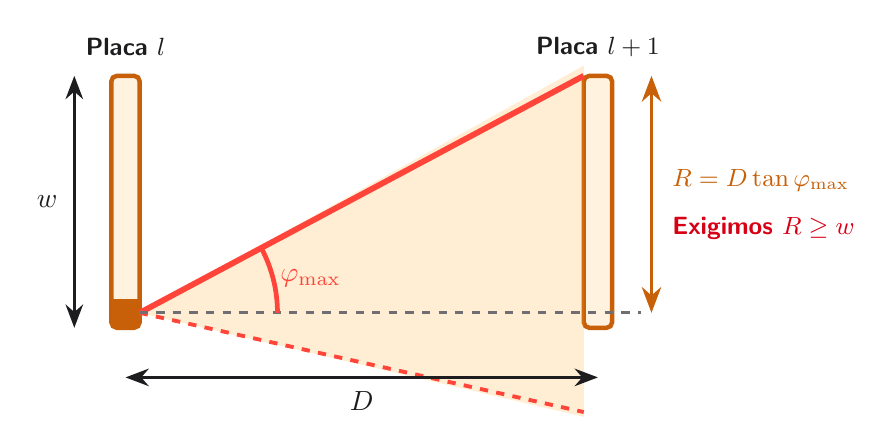
\begin{tikzpicture}[font=\sffamily,>=Stealth]

% Placa l y Placa l+1 de alto w = 3.2 cm (de y=1.35 a y=4.55)
\node[font=\sffamily\small\bfseries,text=ink] at (1.50,4.92) {Placa $l$};
\filldraw[fill=amberfill,draw=amber,line width=1.6pt,rounded corners=2pt]
  (1.32,1.35) rectangle (1.68,4.55);

% Píxel emisor en borde inferior de Placa l
\fill[amber] (1.32,1.35) rectangle (1.68,1.72);

\node[font=\sffamily\small\bfseries,text=ink] at (7.50,4.92) {Placa $l+1$};
\filldraw[fill=amberfill,draw=amber,line width=1.6pt,rounded corners=2pt]
  (7.32,1.35) rectangle (7.68,4.55);

% Centro de emisión en borde inferior (1.68, 1.54)
\coordinate (emit) at (1.68,1.54);

% Cono de difracción que alcanza exactamente el borde superior (7.32, 4.55)
\fill[amberbright,opacity=0.18]
  (emit) -- (7.32,4.68) -- (7.32,0.22) -- cycle;

\draw[redbright,line width=2.1pt] (emit) -- (7.32,4.55);
\draw[redbright,dashed,line width=1.4pt] (emit) -- (7.32,0.28);
\draw[muted,dashed,line width=1.1pt] (emit) -- (8.05,1.54);

% Ángulo phi_max
% Pendiente (4.55-1.54)/(7.32-1.68) = 3.01/5.64 -> atan2 = 28.1 grados
\draw[redbright,line width=1.7pt] (emit) ++(0:1.75) arc (0:28.1:1.75);
\node[font=\sffamily\normalsize\bfseries,text=redbright] at (3.85,1.98) {$\varphi_{\max}$};

% Cota w a la izquierda
\draw[<->,ink,line width=1.2pt] (0.85,1.35) -- (0.85,4.55);
\node[anchor=east,font=\sffamily\normalsize\bfseries,text=ink] at (0.76,2.95) {$w$};

% Cota D debajo
\draw[<->,ink,line width=1.2pt] (1.50,0.72) -- (7.50,0.72);
\node[below,font=\sffamily\normalsize\bfseries,text=ink] at (4.50,0.66) {$D$};

% Cota R = D tan(phi_max) a la derecha
\draw[<->,amber,line width=1.4pt] (8.18,1.54) -- (8.18,4.55);
\node[anchor=west,font=\sffamily\small\bfseries,text=amber,align=left] at (8.32,3.22)
  {$R = D\tan\varphi_{\max}$};
\node[anchor=west,font=\sffamily\small\bfseries,text=red] at (8.32,2.62)
  {Exigimos $R \ge w$};

\end{tikzpicture}
\end{document}
